\def\pgfsysdriver{pgfsys-dvisvgm.def}
\documentclass[tikz,border=5pt]{standalone}

\usepackage{tikz-feynman}
\usepackage[fontset=none]{ctex}
\setCJKsansfont[Path=C:/Windows/Fonts/]{NotoSansSC-VF.ttf}

\definecolor{qftink}{HTML}{26363F}
\definecolor{qftmuted}{HTML}{657B85}
\definecolor{qftsakura}{HTML}{D86483}

\tikzfeynmanset{compat=1.1.0}
\tikzset{
  qft scalar/.style={draw=qftink, line width=0.8pt},
  qft vertex/.style={circle, fill=qftsakura, draw=qftsakura,
    inner sep=1.35pt},
  topology label/.style={font=\sffamily\footnotesize, text=qftmuted},
  point label/.style={font=\small, text=qftink},
}

\begin{document}
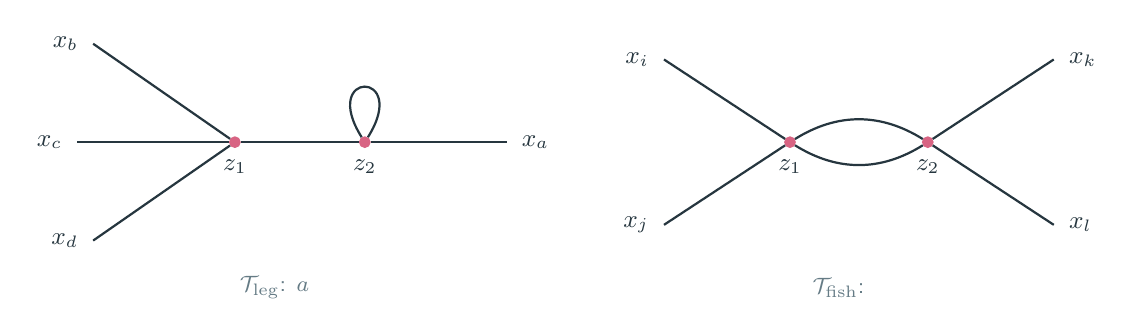
\begin{tikzpicture}[x=1cm, y=1cm]
  \begin{scope}[shift={(0,0)}]
    \begin{feynman}
      \vertex (x1) at (0,1.25);
      \vertex (x2) at (-0.2,0);
      \vertex (x3) at (0,-1.25);
      \vertex[qft vertex] (z1) at (1.8,0) {};
      \vertex[qft vertex] (z2) at (3.45,0) {};
      \vertex (xa) at (5.25,0);
      \diagram*{
        (x1) -- [qft scalar] (z1),
        (x2) -- [qft scalar] (z1),
        (x3) -- [qft scalar] (z1),
        (z1) -- [qft scalar] (z2) -- [qft scalar] (xa)
      };
    \end{feynman}
    \draw[qft scalar] (z2) .. controls +(0.58,0.92) and +(-0.58,0.92) .. (z2);
    \node[point label, left=2pt] at (x1) {$x_b$};
    \node[point label, left=2pt] at (x2) {$x_c$};
    \node[point label, left=2pt] at (x3) {$x_d$};
    \node[point label, right=2pt] at (xa) {$x_a$};
    \node[point label, below=3pt] at (z1) {$z_1$};
    \node[point label, below=3pt] at (z2) {$z_2$};
    \node[topology label] at (2.55,-1.85)
      {$\mathcal T_{\mathrm{leg}}$: $a$ 的四种选择};
  \end{scope}

  \begin{scope}[shift={(7.25,0)}]
    \begin{feynman}
      \vertex (xi) at (0,1.05);
      \vertex (xj) at (0,-1.05);
      \vertex[qft vertex] (z1) at (1.6,0) {};
      \vertex[qft vertex] (z2) at (3.35,0) {};
      \vertex (xk) at (4.95,1.05);
      \vertex (xl) at (4.95,-1.05);
      \diagram*{
        (xi) -- [qft scalar] (z1),
        (xj) -- [qft scalar] (z1),
        (z1) -- [qft scalar, bend left=32] (z2),
        (z1) -- [qft scalar, bend right=32] (z2),
        (z2) -- [qft scalar] (xk),
        (z2) -- [qft scalar] (xl)
      };
    \end{feynman}
    \node[point label, left=2pt] at (xi) {$x_i$};
    \node[point label, left=2pt] at (xj) {$x_j$};
    \node[point label, right=2pt] at (xk) {$x_k$};
    \node[point label, right=2pt] at (xl) {$x_l$};
    \node[point label, below=3pt] at (z1) {$z_1$};
    \node[point label, below=3pt] at (z2) {$z_2$};
    \node[topology label] at (2.48,-1.85)
      {$\mathcal T_{\mathrm{fish}}$: 三个配对道};
  \end{scope}
\end{tikzpicture}
\end{document}
